\documentclass[11pt]{article}
%
% definitions
\usepackage{parskip}
\usepackage{amsmath,amssymb}
\usepackage{xcolor}
\usepackage{bm}
\usepackage{todonotes}
\usepackage{draftwatermark}
\setlength{\marginparwidth}{0.6in} % Needed for todonotes because geometry package is used
\usepackage[vlined,boxed]{algorithm2e}    % For those with brand new LaTeX

\newcommand{\cads}{a}
\newcommand{\eff}{\mathrm{eff}}
\newcommand{\cmax}{c_{\max}}
\newcommand{\Sb}{{\bm{S}}}
\newcommand{\cb}{{\bm{c}}}
\newcommand{\Kb}{{\bm{K}}}
\newcommand{\kb}{{\bm{k}}}
\newcommand{\nb}{{\bm{n}}}
\newcommand{\ub}{{\bm{u}}}
\newcommand{\abs}[1]{\left| #1\right|}
\newcommand{\norm}[1]{\left\| #1\right\|}
\newcommand{\dd}{\mathrm{d}}
\newcommand{\Sdpv}{\ensuremath{S_\text{dpv}}}
\newcommand{\fracpar}[2]{\frac{\partial #1}{\partial #2}}
\newcommand{\code}[1]{\texttt{#1}}

%% Extra markup for revisions:
%\newcommand{\rev}[1]{\textcolor{BrickRed}{#1}}

\title{Equelle Reference Manual}
\author{Atgeirr Fl{\o} Rasmussen, SINTEF ICT}

\begin{document}

\maketitle

\newpage

\tableofcontents

\newpage

%%%%%%%%%%%%%%%%%%%%%%%%%%%%%%%%%%%%%%%%%%%%%%%%%%%%%%%%%%%%%%%%%%%%%%%%%%%%%%
\section{Introduction}

Equelle is a domain-specific language intended for writing simulators, in the sense of
programs that numerically solve partial differential equations. The language was created
at SINTEF ICT, department of Applied Mathematics, starting in 2013.

\subsection{Motivation}

The primary motivation for Equelle is to separate the concerns of the application expert
who knows a field, its physics and equations from the computational scientist who knows
parallel programming and linear solvers.

We also seek to minimize the work needed to port simulators to new architectures and
hardware types. This is achieved by allowing multiple back-ends to the language, reducing
the question of supporting a new hardware type to implementing a new back-end.

We have chosen not to start at the level of the PDEs themselves. Instead, our intention is
that Equelle should make it easy to express the discrete equations for a simulator.
Furthermore, we have concentrated on features useful for finite volume methods, as such
methods are our primary focus.

\subsection{Basic syntax}

An Equelle program consists of a sequence of statements. Statements are terminated by
newlines, unless preceded by an ellipsis (three periods, \code{...}). Comments starts with
the hash character \code{\#} and run to the end of the line, and an ellipsis does not make
the comment continue to the next line. Blocks such as function bodies or \code{For} loop
bodies are delimited by curly brackets (\code{\{ \}}).

\subsection{Vectorized notation}

In languages like C or Fortran, numerical programs usually have a large number of
loops. In Equelle we seek to have fewer loops, and especially to avoid indexing. Indexing
is a major source of errors in numerical computation, and we have sought to minimize them
by using vectorized notation. In Equelle, the statement \code{a = b + c*d} can just as
well refer to collections of number as to single numbers. All such statements are
interpreted element-wise, similar to Matlab's initial-point operators such as
\code{.*} or \code{./} which do not perform matrix operations but element-wise
operations.

\subsection{The grid concept in Equelle}

In any Equelle program, a computational grid is assumed to exist. It is constant and
unchanging from the view of the program, and it is up to the back-end to actually
create or read a particular grid, when the simulator is run.

Grids are cell complexes. They consist of entities of varying dimensionality. The entities
of highest dimension are called cells and all other entities can be obtained as
intersections of cells. The converse also holds: all possible intersections of cells are
entities of the grid. This means that Equelle grids are unstructured, and capable of
representing almost arbitrary computational grids. It also means that there is no notion
of non-conforming grid, since all cell-cell intersections are by definition entities of
the grid.

\subsection{The \code{Collection Of} types}

In most programming languages, a collection of data will be accessed either as a sequence,
or by random access, using indices. In Equelle, data will often be associated with a
subset of grid entities instead. A variable can be created that has one element per cell
in the grid, for example. The Equelle compiler ensures that such a variable cannot be used
in a context where it does not make sense, such as adding it to a variable containing one
element per face. An Equelle \code{Collection} always has a domain, and can be thought of
as a 1-1 mapping from that domain to the data. In traditional languages, such mappings
would implicitly be from the integer indices to the data. New domains can be created from
user input, to capture concepts such as applying a certain boundary condition to only part
of the boundary, or using different equations on part of the grid. There is also a set of
operators (\code{On}, \code{Extend}) that manipulates these mappings, giving a great deal
of flexibility without the risk of indexing errors. The \code{On} concept is described in more
detail in section \ref{subsec:domains-on}.

\subsection{Type checking and type inference}

Equelle is strongly typed. Making a mistake in typing will usually cause a compile
error. This is a safety feature, and when combined with the domains of collections being
part of its type it is a strong safeguard against errors that are easy to make in other
languages.

Mostly, Equelle can be said to be statically typed. However, the domains of
\code{Collection}s can be dynamically computed or input, so that part of the type system
can be said to be dynamic. However, this is all checked at compile time.

\subsection{Declaration and assignment, immutability}

Unlike languages like C++ (at least before \code{auto} was allowed), the user is usually
not burdened with declaring the types of variables. The Equelle compiler is able to infer
the correct types of any valid expression. Therefore Equelle statements can be very
concise, yet unlike languages such as Python or Matlab, type safety is enforced at compile
time.

To declare a variable, use a single statement with a colon separating the variable name
and its type:

\begin{verbatim}
volume : Scalar
\end{verbatim}

To assign a variable, use the \code{=} sign:

\begin{verbatim}
volume = 5.67
\end{verbatim}

This can be combined, as follows:

\begin{verbatim}
volume : Scalar = 5.67
\end{verbatim}

The declarations are entirely optional. They can be included as a form of documentation,
or left out according to the wishes of the programmer. There is an important restriction
on variable and function names: user-declared names must start with a lower case
letter. Names starting with a capital letter are reserved for Equelle. In the remainder of
the name, any letter or number can be used, or underscores.

By default, Equelle variables are immutable, and can only be assigned to once. This makes
it easier for the compiler and back-end to parallelize programs correctly. It is possible
to create mutable variables, but it must be done explicitly, but declaring the variable to
be \code{Mutable}.



%%%%%%%%%%%%%%%%%%%%%%%%%%%%%%%%%%%%%%%%%%%%%%%%%%%%%%%%%%%%%%%%%%%%%%%%%%%%%%
\section{Types in Equelle}

\subsection{Basic types}

There are 7 basic types in Equelle, as shown in Table \ref{tab:basic-types}. Note that
there is no separate type for integer numbers. This helps avoiding some types of errors
that are widespread in other languages, for example the expression \code{1/2} will
yield an expression of type \code{Scalar} with the value 0.5, and not zero as in C.

Vectors are special in that the number of elements will depend on the number of grid
dimensions. A simulator can be created (depending on the back-end used) that is capable of
running simulations on both 2D and 3D grids, and the Vector class will be appropriately
sized in both cases. One can obtain the Scalar elements of a Vector by indexing (starting
from 0):

\begin{verbatim}
a : Vector
...
b : Scalar = a[0]    # First ('x') element.
c : Scalar = a[2]    # Third ('z') element.
\end{verbatim}

Use of vector indexing is checked, and a program that uses the index 2 like in the
assignment of c above, will impose the restriction on the resulting simulator that it
requires 3 grid dimensions.

\begin{table}
\begin{tabular}{l|l}
{\em Type} & {\em Semantics} \\
\hline
\code{Scalar} & A single floating-point number \\
\code{Vector} & A pair or triple of \code{Scalar}s (depending on grid dimension) \\
\code{Bool} & A flag that is \code{True} or \code{False} \\
\code{Cell} & A cell entity of the grid \\
\code{Face} & A face entity of the grid \\
\code{Edge} & An edge entity of the grid \\
\code{Vertex} & A vertex entity of the grid \\
\end{tabular}
\caption{Basic types in Equelle}
\label{tab:basic-types}
\end{table}

\subsection{Collections}

Variable can contain several elements of the same basic type. Such a variable is called a
collection. To declare a collection you use \code{Collection Of} followed by a basic type,
the keyword \code{On} and an expression for the domain of the collection:

\begin{verbatim}
a : Collection Of Scalar On AllFaces()
b : Collection Of Cell On InteriorFaces()
c : Collection Of Vector On AllCells()
\end{verbatim}

Arithmetic operators can be applied only between collections that are \code{On} the same
domain.

\subsection{Domains and the \code{On} concept}
\label{subsec:domains-on}

A domain is defined to be a set of unique grid entities (no repeats), all of the same
dimension. Several basic domains are available via built-in Equelle functions, such as
\code{AllCells()}, \code{BoundaryFaces()} and \code{InteriorVertices()}. It is also
possible to specify domains dynamically, to be set from user input when running a
simulation. For example (including optional type declaration):

\begin{verbatim}
dirichlet_boundary : Collection Of Face Subset Of AllFaces()
dirichlet_boundary =  InputDomainSubsetOf(AllFaces())
\end{verbatim}

This new domain can be used in all ways that the basic built-in domains can. Note that the
\code{Subset Of} part will be discussed in section \ref{subsec:subset-of}.

Given a domain, collections can be declared to be \code{On} that domain. Such a collection
can be thought of as a 1-1 mapping from the domain to the data of the collection. There is
no ordering implicit in this. Consider the following declaration:

\begin{verbatim}
a : Collection Of Scalar On BoundaryFaces()
\end{verbatim}

This can be viewed as mapping taking $f \in \code{BoundaryFaces()} \to a(f)$.

Even if on a low level there exist some ordering of the boundary faces of the grid, it is
not needed by nor accessible from the Equelle program. However, if a different collection
$b$ was declared to be \code{On} the same domain, it would be possible to add or multiply
the collections, and the result would also be \code{On BoundaryFaces()}, for example can
$a + b$ be viewed as mapping taking $f \in \code{BoundaryFaces()} \to a(f) + b(f)$. 

Finally, note that not all collections of grid entities are domains. For example the
collection returned from \code{FirstCell(InteriorFaces())} can possibly contain repeated
instances of one or more cells.

\subsection{The \code{Subset Of} concept}
\label{subsec:subset-of}

It is often necessary to extend or restrict collections to larger or smaller
domains. Therefore it is important to know for any domain, what other domains it is
contained in. For the built-in domains this is obvious and given. For example
\code{BoundaryCells()} is contained within \code{AllCells()}. For domains that are input
from the user, the containing domain must be given as an argument to the
\code{InputDomainSubsetOf()} function, as seen in the \code{dirichlet\_boundary} example
of \ref{subsec:domains-on}.

Given a collection on some domain, one may extend the collection to larger domains by
padding it with zeros. This is only possible for collections of \code{Scalar} type. To do
this one can use the \code{Extend} operator. To continue the previous example:

\begin{verbatim}
x : Collection Of Scalar On dirichlet_boundary
...
y : Collection Of Scalar On BoundaryFaces()
y = x Extend BoundaryFaces()
\end{verbatim}

Similarly, one may do the opposite and restrict a collection to a subdomain by using
\code{On} as an operator:

\begin{verbatim}
x : Collection Of Scalar On BoundaryFaces()
...
y : Collection Of Scalar On dirichlet_boundary
y = x On dirichlet_boundary
\end{verbatim}

A user-specified domain may or may not be a subset of another user-specified domain, but
that is not possible to decide at compile time, and so you can never extend or restrict a
collection from one such domain to another with \code{Extend} and \code{On}
directly. However, it is possible to do so via a containing domain:

\begin{verbatim}
d1 : Collection Of Cell Subset Of AllCells()
d2 : Collection Of Cell Subset Of AllCells()
x1 : Collection Of Scalar On d1
...
x2 = x1 Extend d2                    # Error
x2 = x1 On d2                        # Error
x2 = ((x1 Extend AllCells()) On d2)  # Ok.
\end{verbatim}

The above example first extends x1 with zeros to \code{AllCells()} and then restricts it
to d2. If d2 overlaps d1, then x2 will have the same value as x1 for the cells of d2 that
are also in d1, and zero for the cells that don't.

There is one way the use of \code{On} as an operator is very different from the use of
\code{Extend}: the collection on the right hand side of the \code{On} does not have to be
a domain. Still, all elements of the collection have to be in the domain of the left hand
side. This is looked at in more detail in section \ref{subsec:on-extend}.

\subsection{Sequences}

Unlike a \code{Collection}, that is a mapping from some grid domain, a \code{Sequence} is
a mapping from the integers. It is quite limited what a sequence can be used for,
currently the only usage is to specify the data over which a \code{For} loop iterates. The
declaration syntax for sequences is similar to that for collections, and as with
collections it is possible to have sequences of basic types only. Example usage:
\begin{verbatim}
timesteps : Sequence Of Scalar
timesteps = InputSequenceOfScalar("timesteps")
For dt In timesteps {
    ...
}
\end{verbatim}

The above loop is guaranteed to execute in sequential order, with \code{dt} taking one by
one the values in the sequence \code{timesteps}.

\subsection{Arrays}

First, note that the \code{Array} type is not intended for long arrays. That would be
handled by a \code{Collection} in Equelle. Rather, it is meant to collect small sets of
variables for convenience, especially as function arguments or return types. The size of
an array must be given in the program. It is not possible to use arithmetic operators with
arrays, the only allowed operation is the indexing operation that obtains an element from
the array. Indexing starts from zero. Square brackets can be used to construct an
array. Example usage:
\begin{verbatim}
bothFunc : Function() ...
           -> Array Of 2 Collection Of Cell On InteriorFaces()
bothFunc() = {
    -> [FirstCell(InteriorFaces()), SecondCell(InteriorFaces())]
}
both = bothFunc()
first = both[0]
second = both[1]
wrong = both[2]  # This generates a compiler error
\end{verbatim}

As with access to \code{Vector} types, indexed access is checked by the compiler. If an
expression is an \code{Array} of either \code{Vector} or \code{Collection Of Vector}, the
first indexing operator always refers to elements of the \code{Array}.

\subsection{Function types}

It is a goal to eventually support very flexible function templates in Equelle. However
for now, user-defined functions must have their type declared, meaning that the types of
arguments and the return type must be given. Example usage:

\begin{verbatim}
compRes : Function(u : Collection Of Scalar On AllCells(), ...
                   u0: Collection Of Scalar On AllCells(), ...
                   dt : Scalar) ...
                   -> Collection Of Scalar On AllCells()
\end{verbatim}

Some built-in functions have some polymorphism, such as \code{InputDomainSubsetOf},
\code{Centroid} or \code{Output}. There is at the moment no Equelle syntax that lets the
user create functions with the same flexibility.

\subsection{Mutable variables}

Since variables are immutable by default, they must explicitly be declared mutable. This
is done by writing \code{Mutable} in front of the type. Example usage:

\begin{verbatim}
regular : Scalar = 8
writable : Mutable Scalar = 9
writable = regular  # Ok
writable = 4        # Ok
regular = writable  # Error
regular = 6         # Error
\end{verbatim}


%%%%%%%%%%%%%%%%%%%%%%%%%%%%%%%%%%%%%%%%%%%%%%%%%%%%%%%%%%%%%%%%%%%%%%%%%%%%%%
\section{Built-in operators and functions}

\subsection{Arithmetic operators}

The four fundamental operators (\code{+ - * /}) are available. They can be used with
\code{Scalar} or \code{Vector} expressions, with the exceptions that two \code{Vector}
expressions cannot be multiplied or divided, and that a \code{Scalar} and a \code{Vector}
expression cannot be added or subtracted.

If one expression is a \code{Collection}, then both expressions must be collections that
are \code{On} the same domain. There is one exception to this: you can always multiply or
divide a \code{Collection} with a \code{Scalar}.

The norm operator is written using vertical bars (\code{|}$\cdot$\code{|}) and can be used
for multiple purposes. For a \code{Scalar} it returns the absolute value, for a
\code{Vector} it returns the Euclidean norm, and for grid entities it returns the measure
(volume, area, length) of the entity. It also works for collections, returning a
\code{Collection Of Scalar} in all cases. An example:

\begin{verbatim}
ifaces = InteriorFaces()
first = FirstCell(ifaces)
second = SecondCell(ifaces)
x = |ifaces| * |Centroid(second) - Centroid(first)|
\end{verbatim}

In the above, \code{x} will end up being a \code{Collection Of Scalar On InteriorFaces()},
and its value will be, for each interior face, the product of the face's area with the
distance between its adjacent cells' centroids.


\subsection{Comparisons and logical operators}

The equality comparison operators \code{==} and \code{!=} are accepted by Equelle for all
basic types. The numerical comparisons \code{<}, \code{<=}, \code{>} and \code{>=} are
accepted for \code{Scalar} types only. They all return \code{Bool}, or \code{Collection Of
Bool} if the operands are collections. As for arithmetic operators, both collections must
then be \code{On} the same domain.

The logical operators \code{And}, \code{Or}, \code{Not} and \code{Xor} can be used on
either two \code{Bool} operands or two \code{Collection Of Bool} operands.

The trinary operator (\code{ ? : }) takes three arguments. The first (before the question
mark) must be a \code{Bool}, and the second and third arguments (on either side of the
colon) can be of any type, but both must be of the same type. If the first argument is
true, the second argument is returned, otherwise the third. If any argument is a
collection, they must all be collections on the same domain, and the operator is applied
element-wise.

\subsection{Grid topology}

The built-in functions dealing with grid topology are summarized in Table
\ref{tab:topfunc}. Most of these functions simply return the canonical built-in domains of
Equelle, they all return domains of the indicated type and are named like this:

\code{All|Interior|Boundary + Cells|Faces|Edges|Vertices}.

The functions \code{FirstCell} and \code{SecondCell} do not require domains for their
arguments, nor do they return domains. In a grid, each face is oriented. This orientation
is so that the \code{Normal} of a face points from its \code{FirstCell} to its
\code{SecondCell}. These function may return \code{Empty} for faces on the outer boundary,
in fact the boundary can be characterized by the fact that either \code{FirstCell} or
\code{SecondCell} must be \code{Empty}.

The \code{IsEmpty} function returns \code{True} if the input is \code{Empty} and
\code{False} otherwise.

\begin{table}
\begin{tabular}{l|l|l}
{\em Function} & {\em Arguments} & {\em Returns} \\
\hline
\code{AllCells} & & \code{Collection Of Cell} \\
\code{InteriorCells} & & \code{Collection Of Cell} \\
\code{BoundaryCells} & & \code{Collection Of Cell} \\
\code{AllFaces} & & \code{Collection Of Face} \\
\code{InteriorFaces} & & \code{Collection Of Face} \\
\code{BoundaryFaces} & & \code{Collection Of Face} \\
\code{AllEdges} & & \code{Collection Of Edge} \\
\code{InteriorEdges} & & \code{Collection Of Edge} \\
\code{BoundaryEdges} & & \code{Collection Of Edge} \\
\code{AllVertices} & & \code{Collection Of Vertex} \\
\code{InteriorVertices} & & \code{Collection Of Vertex} \\
\code{BoundaryVertices} & & \code{Collection Of Vertex} \\
\code{FirstCell} & \code{Collection Of Face} & \code{Collection Of Cell}  \\
\code{SecondCell} & \code{Collection Of Face} & \code{Collection Of Cell}  \\
\code{IsEmpty} & \code{Collection Of Cell} & \code{Collection Of Bool}  \\
\end{tabular}
\caption{Grid topology built-in functions}
\label{tab:topfunc}
\end{table}

Consider the following example:

\begin{verbatim}
bfaces = BoundaryFaces()
first = FirstCell(bfaces)
second = SecondCell(bfaces)
bface_cells = IsEmpty(first) ? second : first
\end{verbatim}

The type of \code{bface\_cells} will be \code{Collection Of Cell On BoundaryFaces()}. Note
that some boundary faces can be mapped to the same cell. In the grid in
Figure~\ref{fig:2dgrid} for example, \code{bf\_cells} would contain cell $6$ twice, once for
face $i$ and once for face $u$. Therefore \code{bf\_cells} cannot be a domain.

\begin{figure}
\centering
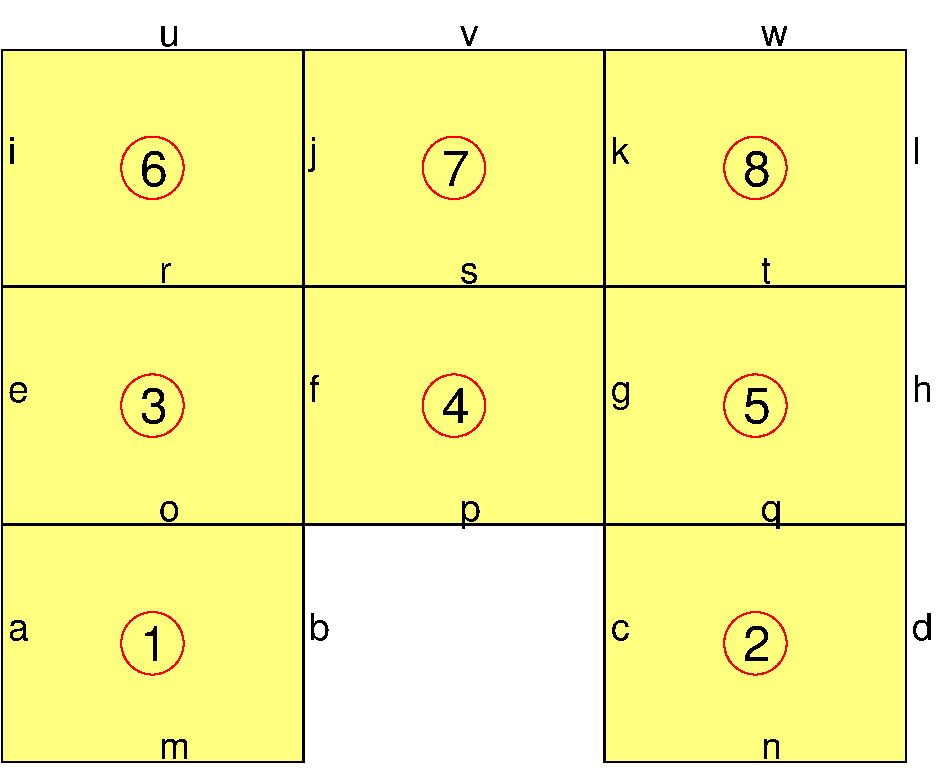
\includegraphics[width=0.8\textwidth]{grid-enumeration}
\caption{An example grid in 2D}
\label{fig:2dgrid}
\end{figure}

\subsection{Grid geometry}

The built-in functions dealing with grid geometry are summarized in Table
\ref{tab:geomfunc}.

\begin{table}
\begin{tabular}{l|l|l}
{\em Function} & {\em Arguments} & {\em Returns} \\
\hline
\code{Centroid} & \code{Collection Of Cell} & \code{Collection Of Vector} \\
\code{Centroid} & \code{Collection Of Face} & \code{Collection Of Vector} \\
\code{Normal} & \code{Collection Of Face} & \code{Collection Of Vector} \\
\end{tabular}
\caption{Grid geometry built-in functions}
\label{tab:geomfunc}
\end{table}

All grid geometry functions return vectors. Note that \code{Normal} returns unit normals.


\subsection{On and Extend as operators}
\label{subsec:on-extend}

The operators \code{On} and \code{Extend} both create new collections from existing
ones. We deal with \code{Extend} first.

\code{Extend} can be used in two ways. The first and simplest is to create a
\code{Collection} from a single (non-collection) expression of a basic type, each element
of the resulting collection being equal to the given single expression. For example we can
extend a previous example:

\begin{verbatim}
bfaces = BoundaryFaces()
first = FirstCell(bfaces)
second = SecondCell(bfaces)
bface_cells = IsEmpty(first) ? second : first
bface_sign = IsEmpty(first) ? (-1 Extend bfaces) : (1 Extend bfaces)
\end{verbatim}

In the above example, \code{(-1 Extend bfaces)} is a \code{Collection Of Scalar On bfaces}
with each element equal to -1. The right hand side expression of the \code{Extend}
operator must be a domain.

The second way to use \code{Extend} is to take a \code{Collection Of Scalar} and extend it
with zeros to form a new \code{Collection Of Scalar} on a larger domain. For example:

\begin{verbatim}
a = AllFaces()
b = BoundaryFaces()
c = Centroid(b)[0]  # The x coordinate of the face centroid
d = x Extend a
\end{verbatim}

A collection can be thought of as a 1-1 mapping from its domain to its data elements. In
the above example, $c$ can be considered to take $f \in b \to c(f)$. Then $d$ takes $f \in
b \to c(f)$ and $f \in a\setminus b \to 0$. For this use of \code{Extend}, the expression
on the right of the operator must be a domain that contains the domain of the collection
of the left.

The \code{On} operator performs the evaluate-on or restrict-to operation on a
collection. Given a collection, one can use \code{On} to form a new collection that is
restricted to a subset of the domain of the original collection. For example:

\begin{verbatim}
all_centroids = Centroid(AllFaces())
boundary_centroids : Collection Of Vector On BoundaryFaces()
boundary_centroids = all_centroids On BoundaryFaces()
\end{verbatim}

In the above, \code{boundary\_centroids} would be identical to the result of
\code{Centroid(BoundaryFaces())}. Note that when unlike \code{Extend}, the \code{On} operator
can be used with other basic types than \code{Scalar}, since it does not need to assign a
default value (zero for \code{Extend}) to any elements, but draws all its data from the
collection given on the left hand side. The new collection's domain will be the same as
that of the right hand side.

The right hand side does not need to be a domain in itself. It is however required to be a subset of
the domain of the left hand side collection. Extending a previous example shows how:

\begin{verbatim}
bfaces = BoundaryFaces()
first = FirstCell(bfaces)
second = SecondCell(bfaces)
bface_cells = IsEmpty(first) ? second : first
bface_cell_centroids = Centroid(AllCells()) On bface_cells
\end{verbatim}

In the above, the type of \code{bface\_cells} is \code{Collection Of Cell On
  BoundaryFaces() Subset Of AllCells()}. It contains, for each boundary face, the cell
just on the inside of the face. It is not a domain, since any cell can occur multiple
times in the collection. The collection \code{bface\_cell\_centroids} contains, for each
boundary face, the centroid of the cell just inside of it.

Another example:

\begin{verbatim}
a = AllCells()
c = Centroid(a)
s = SecondCell(InteriorFaces())
d = c On s
\end{verbatim}


Viewing collections as 1-1 mappings from domains to data, one can say that if $c$ takes an
element $e \in a \to c(e)$ and $s \subset a$, then $d$ (which is given by \code{c On s})
simply takes $e \in s \to c(e)$.

\subsection{Discrete operators}

The discrete operators \code{Gradient} and \code{Divergence} make it easy to program
finite volume methods. Their properties are summarized in Table~\ref{tab:discops}.

\begin{table}[h]
\begin{tabular}{l|p{4.5cm}|p{4.5cm}}
{\em Function} & {\em Arguments} & {\em Returns} \\
\hline
\code{Gradient} & \code{Collection Of Scalar On AllCells()}
& \code{Collection Of Scalar On InteriorFaces()} \\
\code{Divergence} & \code{Collection Of Scalar On InteriorFaces()}
& \code{Collection Of Scalar On AllCells()} \\
\code{Divergence} & \code{Collection Of Scalar On AllFaces()}
& \code{Collection Of Scalar On AllCells()} \\
\end{tabular}
\caption{Discrete operators}
\label{tab:discops}
\end{table}

The function call \code{Gradient(x)} computes for each interior face, the difference
between \code{x} at the two adjacent cells. It is equivalent to the following Equelle
function:

\begin{verbatim}
grad : Function(x : Collection Of Scalar On AllCells()) ...
                -> Collection Of Scalar On InteriorFaces()
grad(x) = {
    first = FirstCell(InteriorFaces())
    second = SecondCell(InteriorFaces())
    -> (x On second) - (x On first) 
}
\end{verbatim}

The function call \code{Divergence(x)} computes for each cell, the discrete divergence of
the flux \code{x}. This is equal to the orientation-signed sum of the elements of \code{x}
belonging to faces adjacent to the cell. This sum is done with signs, in such a way that
elements of faces that are positively oriented with respect to the cell are added, and
elements with negative orientation subtracted. Consider for example the grid in
Figure~\ref{fig:2dgrid}. Assume that all faces are oriented so that the normals point to
the right or upwards. Then the (signed) boundary of cell 3 is equal to $-e + f - o +
r$. If those faces have associated fluxes equal to $\{0, 1, 2, -1\}$ the divergence at
cell 3 would be $-0 + 1 - 2 + (-1) = -2$.

Note that there are two variants of \code{Divergence}: for convenience there is one that
is defined on \code{InteriorFaces()} only, it is equivalent to the following function
invoking the full \code{Divergence} function:

\begin{verbatim}
div_int : Function(x : Collection Of Scalar On InteriorFaces()) ...
                   -> Collection Of Scalar On AllCells()
div_int(x) = {
    -> Divergence(x Extend AllFaces())
}
\end{verbatim}

It is not possible to define an Equelle function that is equivalent to the full
\code{Divergence} built-in function, since there is no way (for now at least) to access
the neighbour faces of a cell.

\subsection{Solver functions}

Equelle is not intended to write advanced linear solvers or similar low-level
code. Instead, such features are meant to be provided by the back-end, through solver
functions of the language. So far, there are only 2 such functions available, for solving
nonlinear (or linear) problems with the Newton-Raphson method.

The simplest, \code{NewtonSolve}, solves a scalar equation. It takes as arguments a
function and an initial guess, and returns a value that makes the function zero within
some tolerance. What that tolerance is and how it is controlled is currently up to the
back-end to specify. Since Equelle does not have a system for exceptions or other error
handling, it is back-end dependent what happens if the algorithm fails to converge. The
function argument, its return value, and the initial guess must all be of the same type,
scalar collections over the same domain. A short example:

\begin{verbatim}
pressureResLocal(pressure) = {
    -> computePressureResidual(pressure, total_mobility, source)
}
p = NewtonSolve(pressureResLocal, p0)
\end{verbatim}

In the above, there exists some function \code{computePressureResidual} taking three
arguments. At the point shown we want to solve for the first argument, with fixed values
for the two other arguments. We then create a local function binding the two last
arguments, and pass the resulting function to \code{NewtonSolve} together with an initial
guess.

For systems of equations \code{NewtonSolveSystem} is available. Its interface is very
similar to the simple version. It takes as argument an \code{Array Of} functions and an
\code{Array Of} initial guesses, and returns an \code{Array Of} solutions:

\begin{verbatim}
pressureResLocal : Function(pressure : Collection Of Scalar On AllCells(), ...
                            sw : Collection Of Scalar On AllCells()) ...
                            -> Collection Of Scalar On AllCells()
pressureResLocal(pressure, sw) = {
    total_mobility = computeWaterMob(sw) + computeOilMob(sw)
    -> computePressureResidual(pressure, total_mobility, source)
}

newvals = NewtonSolveSystem([pressureResLocal, transportResLocal], ...
                            [p0, 0.5 Extend AllCells()])
\end{verbatim}

In the above partial example, we want to solve for \code{pressure} and \code{sw}
simultaneously. Then we have to pass arrays to \code{NewtonSolveSystem}, and each of those
functions needs to take both of the unknowns as inputs, as shown above for the
\code{pressureResLocal} function. The \code{transportResLocal} function is not shown here,
but that one also must take both \code{pressure} and \code{sw}.

\subsection{Input and output}

Equelle provides function to get user input, that are summarized in
Table~\ref{tab:iofunc}. All functions take a \code{String} argument, a tag for the
operation. It is up to the back-end how that is used, for example the serial back-end
writes a series of numbered files prefixed with the tag each time \code{Output} is called
with the same tag. The function \code{InputCollectionOfScalar} takes a domain as input,
and returns a collection over the same domain. The function \code{InputDomainSubsetOf}
takes a domain as input argument, and returns a new domain that is a subset of the input
domain. Ensuring that any user input actually satisfies this is the duty of the
back-end. This function is notable in particular, since it is the only way to create a new
domain that is not equal to one of the 12 standard domains (\code{AllCells(),
InteriorCells()} etc.).

\begin{table}
\begin{tabular}{l|l|l}
{\em Function} & {\em Arguments} & {\em Returns} \\
\hline
\code{InputScalarWithDefault} & \code{String, Scalar} & \code{Scalar} \\
\code{InputCollectionOfScalar} & \code{String}, {\em domain} & \code{Collection Of Scalar} \\
\code{InputDomainSubsetOf} & \code{String}, {\em domain} & {\em domain} \\
\code{InputSequenceOfScalar} & \code{String} & \code{Sequence Of Scalar} \\
\code{Output} & \code{String, Scalar} & \\
\code{Output} & \code{String, Collection Of Scalar} & \\
\end{tabular}
\caption{I/O functions}
\label{tab:iofunc}
\end{table}

\subsection{Miscellaneous functions}

Other built-in functions include the dot product, \code{Dot}, and the square root
function, \code{Sqrt}. See Table~\ref{tab:miscfunc} for a summary.

\begin{table}
\begin{tabular}{l|l|l}
{\em Function} & {\em Arguments} & {\em Returns} \\
\hline
\code{Dot} & 2 \code{Collection Of Vector}s & \code{Collection Of Scalar} \\
\code{Sqrt} & \code{Collection Of Scalar} & \code{Collection Of Scalar} \\
\end{tabular}
\caption{Miscellaneous functions}
\label{tab:miscfunc}
\end{table}

%%%%%%%%%%%%%%%%%%%%%%%%%%%%%%%%%%%%%%%%%%%%%%%%%%%%%%%%%%%%%%%%%%%%%%%%%%%%%%
% \section{Control structures and user-defined functions}

% \subsection{Scopes}

% \subsection{The For construct}

% \subsection{Functions}


% %%%%%%%%%%%%%%%%%%%%%%%%%%%%%%%%%%%%%%%%%%%%%%%%%%%%%%%%%%%%%%%%%%%%%%%%%%%%%%
% \section{The grammar of Equelle}

% \subsection{Allowed identifiers}

% \subsection{Syntax for literals}

% \subsection{Expression syntax}

% \subsection{Statements}

% \subsection{The formal grammar definition}


%%%%%%%%%%%%%%%%%%%%%%%%%%%%%%%%%%%%%%%%%%%%%%%%%%%%%%%%%%%%%%%%%%%%%%%%%%%%%%
% Bibliography.

%\begin{small}
%  \bibliographystyle{spelike} %\bibliography{bib/polymer,bib/diagnostics,bib/co2,bib/fronttracking,bib/divSINTEF,bib/reorder,bib/streamlines,bib/misc}
%\end{small}


\end{document}


%% Local Variables:
%% fill-column: 90
%% mode: LaTeX
%% TeX-master: t
%% End:
